\PassOptionsToPackage{table}{xcolor}
\PassOptionsToPackage{svgnames}{xcolor}
\documentclass[utf8,stillsansserifmath,fleqn,t]{beamer}
\usepackage[english]{babel}
\usepackage{graphicx}
\usepackage{amsmath}
\usepackage[overlay]{textpos}
\usepackage{helvet}
\usepackage{ifthen}
\usepackage{listings}
\usepackage[utf8]{inputenc}
\usepackage[T1]{fontenc}

% Select beamer theme
\mode<presentation>{\usetheme{CG}}
\usefonttheme[onlymath]{serif}
%\textblockorigin{0pt}{0pt}
\setlength{\TPHorizModule}{\textwidth}
\setlength{\TPVertModule}{\textheight}

% In-text code sample
\newcommand{\code}[1]{\texttt{#1}}
% Larger code examples with lstlisting
\lstloadlanguages{C}
\lstdefinelanguage[OpenGL]{C}[ANSI]{C}{%
    morekeywords={bool,bvec2,bvec3,bvec4,ivec2,ivec3,ivec4,vec2,vec3,vec4}
}
\lstset{%
    language=[OpenGL]C,
    basicstyle=\footnotesize\ttfamily,%
    keywordstyle=\color{cgblue},%
    directivestyle=\color{cgblue},%
    identifierstyle=,%
    commentstyle=\color{cgblue!50!white}\itshape,%
    stringstyle=\color{cgblue!80!white},%
    numbers=none,%
    numberstyle=\tiny,%
    extendedchars=true,%
    showspaces=false,%
    showstringspaces=false,%
    showtabs=false,%
    breaklines=false,%
    frame=single,%
    frameround=tttt,%
    backgroundcolor=\color{cgblue!10!white},%
    escapechar=\%
}

% Random useful stuff
\newcommand{\ds}{\displaystyle}
\usepackage{pifont}
\newcommand{\cmark}{\ding{51}}%
\newcommand{\xmark}{\ding{55}}%

% Links
\hypersetup{colorlinks,linkcolor=,urlcolor=blue}

% Title page
\title[Virtual Reality Application Programming with QVR]
{Virtual Reality Application Programming\\with QVR}
\author[M. Lambers]%
{\href{http://www.cg.informatik.uni-siegen.de/}{Computer Graphics and\\
Multimedia Systems Group}\\~\\
\href{http://www.uni-siegen.de}{University of Siegen}}
\institute[University of Siegen]{~}
\date{\today}
\titlegraphic{%

\includegraphics[height=8ex]{logo-cg.pdf}\hspace{3ex}%

\includegraphics[height=8ex]{logo-uni.pdf}%
}


\begin{document}

\begin{frame}
\titlepage
\end{frame}

\begin{frame}
\frametitle{Overview}
\tableofcontents
\end{frame}

\section{Challenges for VR frameworks}

\begin{frame}
\frametitle{\insertsection}
Challenges
\begin{itemize}
\item VR applications run on a wide variety of graphics and display hardware setups:\\
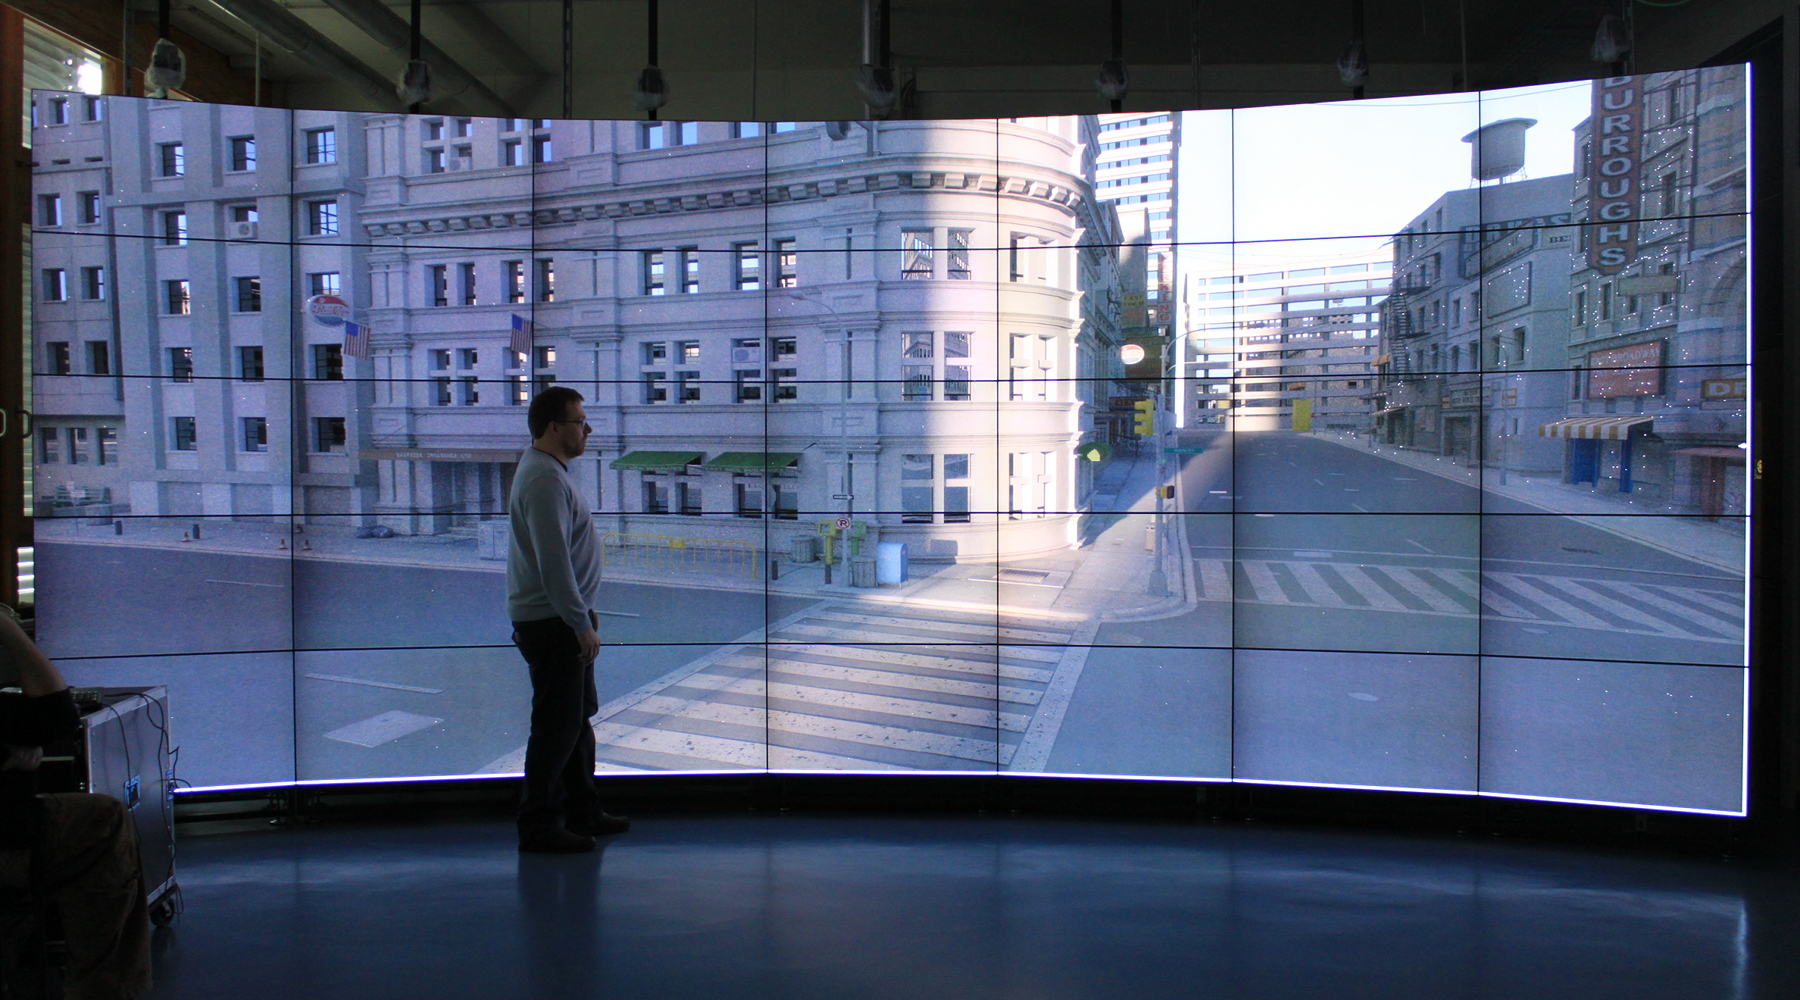
\includegraphics[height=.18\textheight]{./fig/hornet.jpg}~
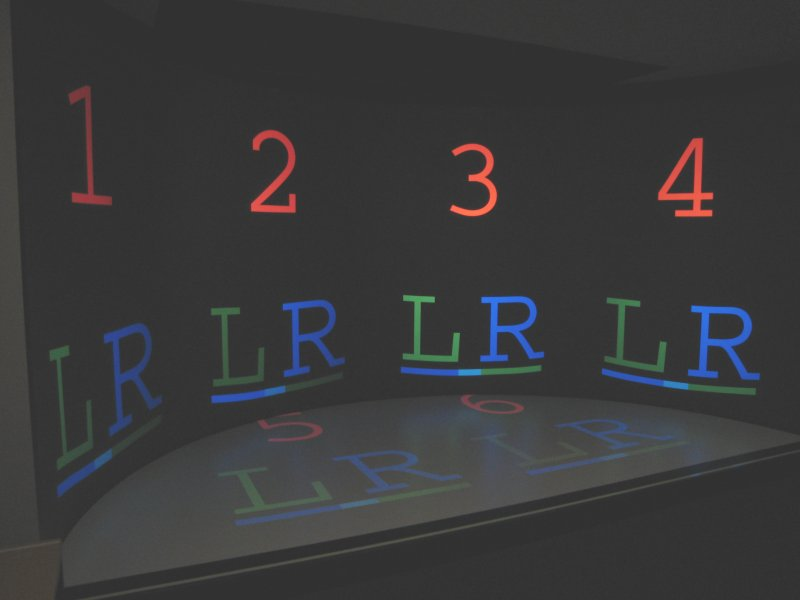
\includegraphics[height=.18\textheight]{./fig/vrlab-unisiegen.jpg}~
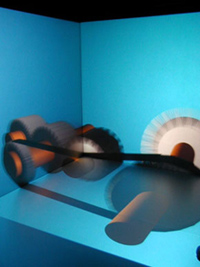
\includegraphics[height=.18\textheight]{./fig/minicave.jpg}~
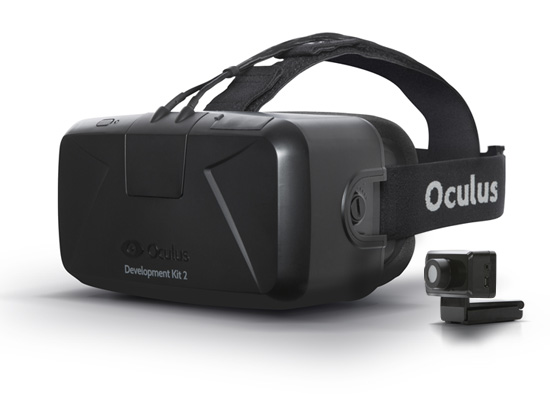
\includegraphics[height=.18\textheight]{./fig/oculus-rift-dk2.jpg}~
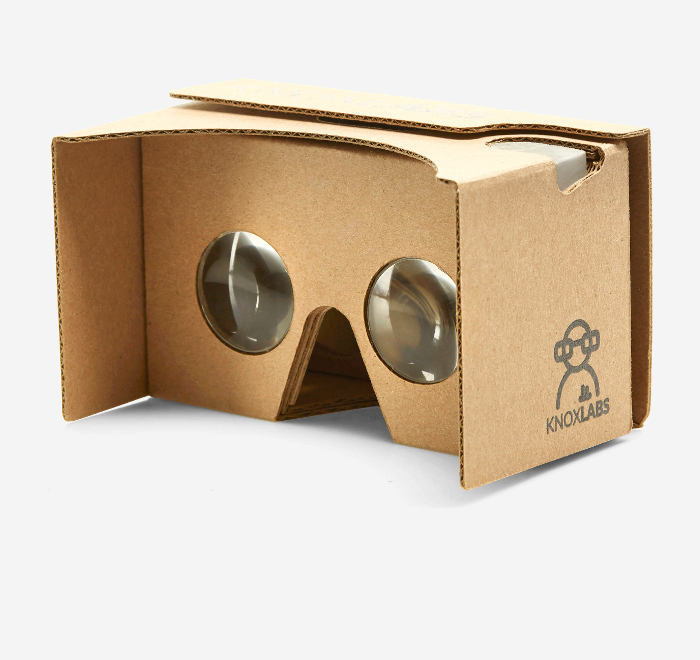
\includegraphics[height=.18\textheight]{./fig/cardboard.jpg}\\
\item In general, a VR application must handle
    \begin{itemize}
    \item Multiple hosts (for render clusters)
    \item Multiple GPUs on a host
    \item Multiple displays devices attached to a GPU
    \end{itemize}
    whereas typical non-VR graphics applications only handle
    \begin{itemize}
    \item A single display device attached to a single GPU on a single host
    \end{itemize}
\end{itemize}
\end{frame}

\begin{frame}
\frametitle{\insertsection}
VR frameworks\\~\\
{\footnotesize
\begin{tabular}{l|c|c|c|c|c|l}
~       & Multi-      & Vive,    & Google  & Allows   & Li-  & ~ \\
~       & GPU \&      & Oculus   & VR      & own      & cense& Remarks \\
~       & Cluster     & ~        & ~       & renderer & ~    & ~\\ \hline
\href{http://doi.org/10.1109/VR.1999.756918}{Avocado} &
           \cmark     & \xmark   & \xmark  & \xmark   & ---  & Dead\\\hline
\href{http://www.vrjuggler.org/}{VRJuggler} &
           \cmark     & \xmark   & \xmark  & ?        & LGPL & Smelling funny\\\hline
\href{http://opensg.org/}{OpenSG} &
           \cmark     & \xmark   & \xmark  & \xmark   & LGPL & Fraunhofer\\\hline
\href{http://www.itc.rwth-aachen.de/cms/IT-Center/Forschung-Projekte/Virtuelle-Realitaet/Infrastruktur/~fgmo/ViSTA-Virtual-Reality-Toolkit/?lidx=1}{ViSTA}&
           \cmark     & \xmark   & \xmark  & (\xmark) & LGPL & RWTH AC \& DLR\\\hline
\href{https://github.com/Eyescale/Equalizer}{Equalizer} &
           \cmark     & (\xmark) & \xmark  & \cmark   & LGPL & More than VR! \\\hline
\href{https://www.unrealengine.com/}{Unreal Eng.} & (\href{http://hci.uni-wuerzburg.de/projects/caveudk/}{\xmark}) 
                      & \cmark   & \cmark  & \xmark   & Propr. & Epic Games\\\hline
\href{https://unity3d.com/}{Unity Eng.} &
           \xmark     & \cmark   & \cmark  & \xmark   & Propr. & Unity Tech.\\\hline
\href{https://marlam.de/qvr}{QVR} &
           \cmark     & \cmark   & (\cmark)  & \cmark   & MIT  & ~\\
\end{tabular}
}
\end{frame}

\begin{frame}
\frametitle{\insertsection}
\centerline{Typical non-VR graphics application}~\\
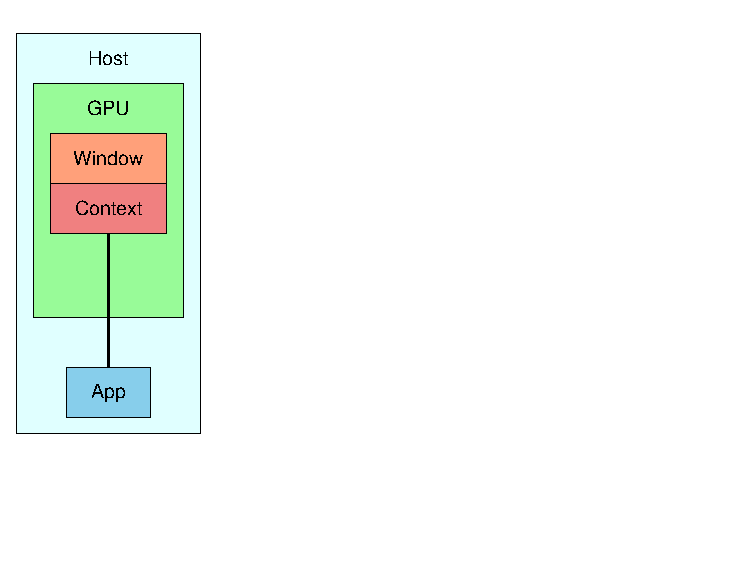
\includegraphics[height=.75\textheight]{./fig/setup-simple.pdf}\\
\vspace*{-.75\textheight}\hspace*{.27\textwidth}\begin{minipage}{.72\textwidth}
\begin{itemize}
\item The application uses a toolkit to create a window
\item The toolkit creates an OpenGL context automatically and ``makes it
current''
\item The application never needs to care about the context
    \begin{itemize}
    \item There is only one context
    \item The context is always current
    \end{itemize}
\end{itemize}
\end{minipage}
\end{frame}

\begin{frame}
\frametitle{\insertsection}
\centerline{VR application using multiple hosts, GPUs, and displays}~\\
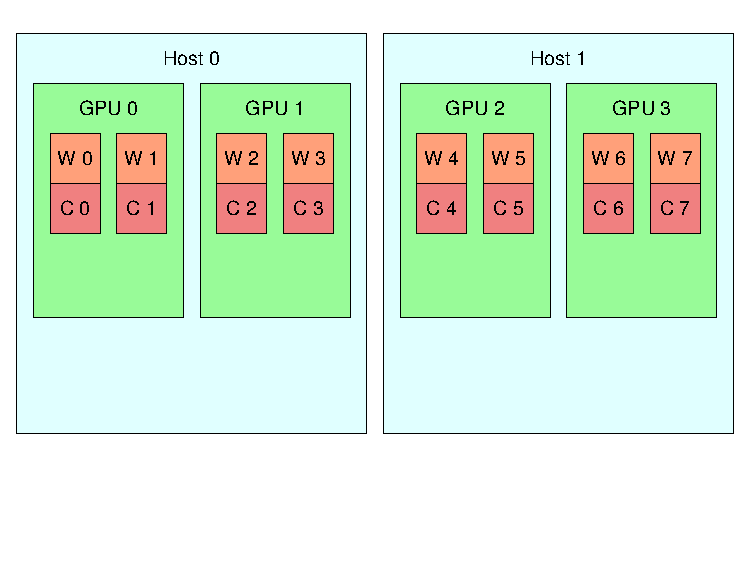
\includegraphics[height=.75\textheight]{./fig/setup-vr-unknown.pdf}
\end{frame}

\begin{frame}
\frametitle{\insertsection}
Challenges: OpenGL contexts and threading
\begin{itemize}
\item OpenGL contexts on the same GPU can \emph{share} objects
such as textures.\\
$\rightarrow$ Only one context should manage OpenGL objects.
\item A context can only be current in one thread at a time, and a
switch of that thread is expensive.\\
$\rightarrow$ All rendering to a context should happen from only one thread.
\item Access to a single GPU is serialized by the driver.\\
$\rightarrow$ Rendering into different contexts on the same GPU should be
serialized to avoid context switches.
\item The function that triggers swapping of back and front buffers 
blocks until the swap happened, and the swap is typically synchronized to the
display frame rate.\\
$\rightarrow$ The thread in which the context is current is often blocked.
\end{itemize}
\end{frame}

\section{Solutions for Multi-GPU / Multi-Host VR}

\begin{frame}
\frametitle{\insertsection}
\centerline{Multi-Context Multi-Thread Approach}~\\
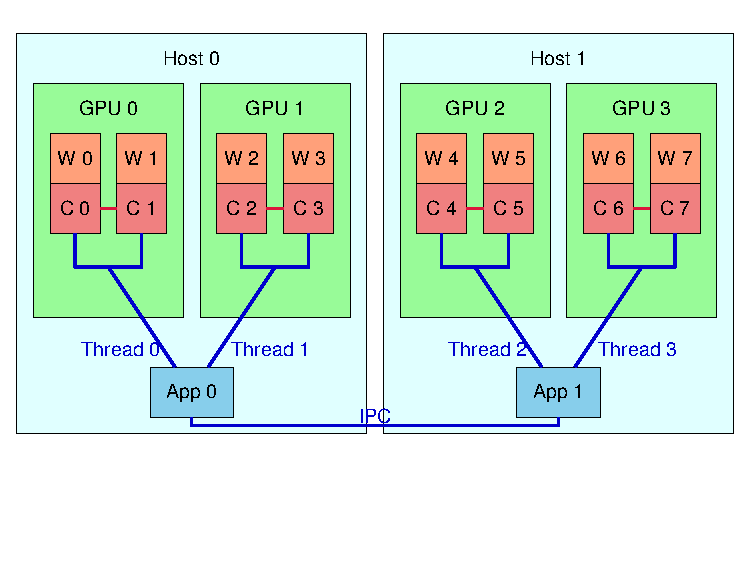
\includegraphics[height=.75\textheight]{./fig/setup-vr-mcmt.pdf}
\end{frame}

\begin{frame}
\frametitle{\insertsection}
Multi-Context Multi-Thread Approach
\begin{itemize}
\item One process per host
\item One context per window
\item One thread per GPU
    \begin{itemize}
    \item Contexts driven by thread share objects
    \item Window views driven by thread are rendered sequentially
    \end{itemize}
\item An application process must be aware of
    \begin{itemize}
    \item Multiple rendering threads
    \item Multiple contexts that may or may not be sharing objects
    \end{itemize}
\item Interprocess communication:
    \begin{itemize}
    \item Only between hosts
    \end{itemize}
\end{itemize}
\end{frame}

\begin{frame}
\frametitle{\insertsection}
\centerline{Single-Context Single-Thread Approach}~\\
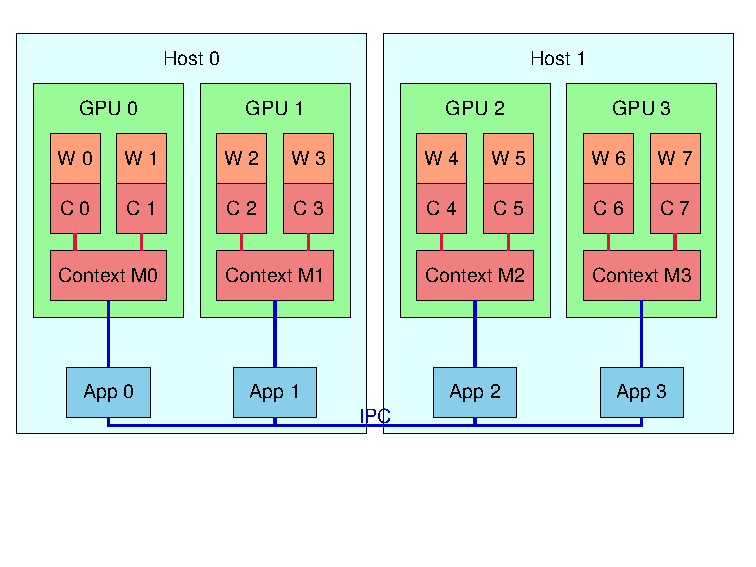
\includegraphics[height=.75\textheight]{./fig/setup-vr-scst.pdf}
\end{frame}

\begin{frame}
\frametitle{\insertsection}
Single-Context Single-Thread Approach
\begin{itemize}
\item One process per GPU
\item One context per process (plus one hidden context per window)
\item One thread per process (main thread)
    \begin{itemize}
    \item Context sharing irrelevant to application
    \item Window views are rendered sequentially
    \end{itemize}
\item An application process must be aware of
    \begin{itemize}
    \item Only one thread (rendering threads are hidden)
    \item Only one context (window contexts are hidden)
    \end{itemize}
\item Interprocess communication:
    \begin{itemize}
    \item Between hosts
    \item Between processes on same host if multiple GPUs are used
    \end{itemize}
\end{itemize}
\end{frame}

\section{QVR Overview and Concepts}

\begin{frame}
\frametitle{\insertsection}
The \href{https://marlam.de/qvr}{QVR} framework
\begin{itemize}
\item Implements the single-context single-thread approach\\ for multi-GPU / multi-host support
\item Based on \href{http://www.qt.io/}{Qt} (requires nothing else)
\item Manages four major types of objects:
    \begin{itemize}
    \item \emph{Devices} used for interaction, e.g. game controllers
    \item \emph{Observers} that view the virtual scene
    \item \emph{Windows} that provide views of the virtual scene
    \item \emph{Processes} that run on hosts and manage windows 
    \end{itemize}
\item A VR application implements a simple interface:
    \begin{itemize}
    \item \emph{render()} to render a view of the scene into a texture
    \item \emph{update()} for interactions, animations, and other scene updates
    \item Optional: one-time or per-frame actions per process or window
    \item Optional: device/keyboard/mouse event handling
    \item Optional: serialization, for multi-process support
    \end{itemize}
\item Applications run unmodified on different setups
\end{itemize}
\end{frame}

\begin{frame}
\frametitle{\insertsection}
\begin{minipage}[t]{.33\textwidth}
    \centerline{Functionality}\vspace{.5\baselineskip}
    \begin{itemize}
    \item Handles tracking\\
    {\footnotesize Glasses / HMDs, Controllers, \ldots{}}
    \item Handles input\\
    {\footnotesize Controller buttons / joysticks, mouse / keyboard}
    \item Handles output\\
    {\footnotesize Puts left/right view onto screen(s) as appropriate}
    \end{itemize}
\end{minipage}\hfill
\begin{minipage}[t]{.33\textwidth}
    \centerline{Application View}\vspace{.5\baselineskip}
    \begin{itemize}
    \item Implements \hbox to 0pt{\code{QVRApp}}\\
    {\footnotesize
        \code{render()}, \code{update()}, \ldots{}
    }
    \item Can access\\
    {\footnotesize
        \code{QVRDevice},
        \code{QVRObserver},
        \code{QVRWindow},
        \code{QVRProcess}
    }
    \item Does not need to care about\\
    {\footnotesize
        VR hardware, Multi-GPU, threads,
        OpenGL contexts,
        \ldots{}
    }
    \end{itemize}
\end{minipage}\hfill
\begin{minipage}[t]{.33\textwidth}
    \centerline{VR System View}\vspace{.5\baselineskip}
    \begin{itemize}
    \item Configuration describes available VR hardware
    \item Autodetected or manually configured
    \item Configuration classes
    {\footnotesize
        \code{QVRDeviceConfig},
        \code{QVRObserverConfig},
        \code{QVRWindowConfig},
        \code{QVRProcessConfig}
    }
    \end{itemize}
\end{minipage}
\end{frame}

\begin{frame}
\frametitle{\insertsection}
Illustration
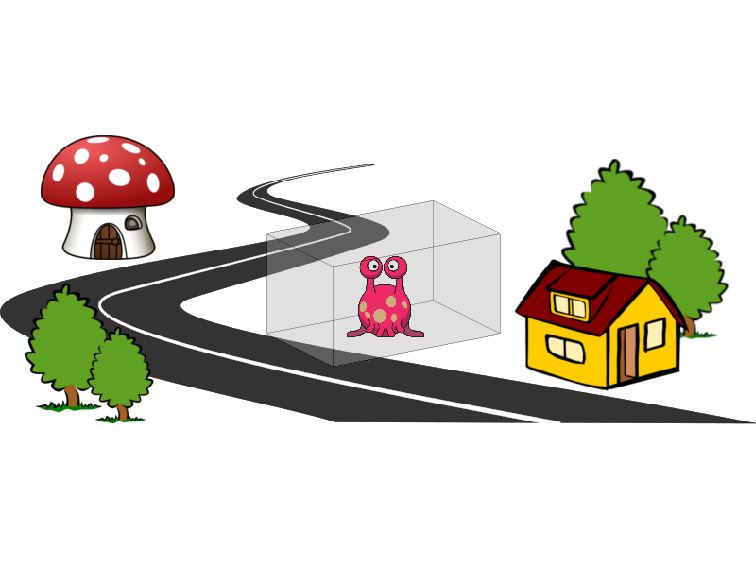
\includegraphics[width=\textwidth]{./fig/scene.pdf}
\vspace*{-4ex}
\begin{itemize}
\item You are an alien
\item Your UFO is a transparent box
\item You fly your UFO through a strange world
\item You can move freely inside your UFO
\end{itemize}
\end{frame}

\begin{frame}
\frametitle{\insertsection}
~\\
\begin{minipage}{0.49\textwidth}
\centerline{Illustration}\vspace{1ex}
\begin{itemize}
\item The alien views the world through the sides of his UFO.\\~\\~
\item The alien flies its UFO through the world.
\item The alien moves inside its UFO.
\end{itemize}
\end{minipage}\hfill
\begin{minipage}{0.49\textwidth}
\centerline{QVR}\vspace{1ex}
\begin{itemize}
\item An \emph{observer} views the virtual world in \emph{windows};
each \emph{window} provides a view for one \emph{observer}.
\item An observer \emph{navigates} through the virtual world.
\item An observer's movements are \emph{tracked} inside a tracking space.
\end{itemize}
\end{minipage}
\end{frame}

\begin{frame}
\frametitle{\insertsection}
Devices (in illustration: for example the UFO remote control)
\begin{itemize}
\item Optional: can be tracked inside a tracking space
\item Optional: provides buttons and other interaction controls
\item Examples:
    \begin{itemize}
    \item Tracked glasses
    \item Traditional game controller
    \item HTC Vive controllers
    \item ART Flystick
    \end{itemize}
\item Configured through \href{https://marlam.de/qvr/libqvr-reference/class_q_v_r_device_config.html}{QVRDeviceConfig}
    \begin{itemize}
    \item Tracking
        \begin{itemize}
        \item Type and parameters (e.g. based on VRPN, Oculus Rift)
        \item Initial position and orientation
        \end{itemize}
    \item Digital buttons
    \item Analog elements (triggers, joysticks, trackpads)
    \end{itemize}
\item Implemented as \href{https://marlam.de/qvr/libqvr-reference/class_q_v_r_device.html}{QVRDevice}
    \begin{itemize}
    \item Tracking: position and orientation
    \item State of buttons and analogs
    \item Accessible to the update() function for interaction
    \end{itemize}
\end{itemize}
\end{frame}

\begin{frame}
\frametitle{\insertsection}
Observer (in illustration: the alien)
\begin{itemize}
\item Views the virtual world through one or more windows
\item Can navigate through the virtual world
\item Can be bound to tracked devices, e.g. glasses
\item Configured through \href{https://marlam.de/qvr/libqvr-reference/class_q_v_r_observer_config.html}{QVRObserverConfig}
    \begin{itemize}
    \item Navigation
        \begin{itemize}
        \item Type and parameters (e.g. based on QVR device interaction)
        \item Initial position and orientation
        \end{itemize}
    \item Tracking
        \begin{itemize}
        \item Type and parameters (e.g. based on specific devices)
        \item Initial position and orientation
        \item Eye distance
        \end{itemize}
    \end{itemize}
\item Implemented as \href{https://marlam.de/qvr/libqvr-reference/class_q_v_r_observer.html}{QVRObserver}
    \begin{itemize}
    \item Navigation: position and orientation
    \item Tracking: position and orientation \emph{for each eye}
    \end{itemize}
\end{itemize}
\end{frame}

\begin{frame}
\frametitle{\insertsection}
Window (in illustration: a side of the box-shaped UFO)
\begin{itemize}
\item Provides a view of the virtual world for exactly one observer
\item Configured through \href{https://marlam.de/qvr/libqvr-reference/class_q_v_r_window_config.html}{QVRWindowConfig}
    \begin{itemize}
    \item Observer to provide a view for
    \item Output mode (left/right/stereo view) and parameters
    \item Geometry in pixels
    \item 3D geometry in the virtual world
        (if the window corresponds to a physical screen wall)
    \end{itemize}
\item Implemented as \href{https://marlam.de/qvr/libqvr-reference/class_q_v_r_window.html}{QVRWindow}
    \begin{itemize}
    \item Accessible as QWindow for the application, if required
    \item Hides its context and rendering thread
    \end{itemize}
\end{itemize}
\end{frame}

\begin{frame}
\frametitle{\insertsection}
Process
\begin{itemize}
\item Provides one OpenGL context to the application
\item Drives zero or more windows
\item Runs one instance of the VR application
\item First process is main process; child processes are started automatically
when needed
\item Configured through \href{https://marlam.de/qvr/libqvr-reference/class_q_v_r_process_config.html}{QVRProcessConfig}
    \begin{itemize}
    \item GPU to use (system specific)
    \item Launcher command (e.g. for network processes)
    \item List of window configurations
    \end{itemize}
\item Implemented as \href{https://marlam.de/qvr/libqvr-reference/class_q_v_r_process.html}{QVRProcess}
    \begin{itemize}
    \item Accessible as QProcess for the application, if required
    \item Hides communication between main and child processes
    \end{itemize}
\end{itemize}
\end{frame}

\section{QVR Application Interface}

\begin{frame}
\frametitle{\insertsection}
Application
\begin{itemize}
\item Interface specified in the \href{https://marlam.de/qvr/libqvr-reference/class_q_v_r_app.html}{QVRApp} class
\item All functions except \code{render()} are optional to implement; the empty
default implementation is sufficient
\item \code{void render(QVRWindow* w, const QVRRenderContext\& context, const
unsigned int* textures)}
    \begin{itemize}
    \item Called once per window per frame
    \item Renders one (mono) or two (stereo 3D) views for window \code{w} into
    \code{textures}
    \item The \code{context} contains all necessary information for the view(s)
    \end{itemize}
\end{itemize}
\end{frame}

\begin{frame}[fragile]
\frametitle{\insertsection}
Application: \code{render()}
\begin{lstlisting}
void render(QVRWindow* w, const QVRRenderContext& context,
            const unsigned int* textures) {
    for (int view = 0; view < context.viewCount(); view++) {
        // Get view dimensions
        int width = context.textureSize(view).width();
        int height = context.textureSize(view).height();
        // Set up framebuffer object to render into texture
        setupFBO(textures[view]);
        // Set up view
        glViewport(0, 0, width, height);
        glClear(GL_COLOR_BUFFER_BIT | GL_DEPTH_BUFFER_BIT);
        QMatrix4x4 P = context.frustum(view).toMatrix4x4();
        QMatrix4x4 V = context.viewMatrix(view);
        // Render
        ...;
    }
}
\end{lstlisting}
\end{frame}

\begin{frame}
\frametitle{\insertsection}
Application (continued)
\begin{itemize}
\item \code{void update(const QList<QVRObserver*>\& observers)}
    \begin{itemize}
    \item Called once before each frame \emph{on the main process}
    \item Updates scene state, e.g. for animations
    \item May update observers, e.g. for navigation
    \item May use QVR devices for interaction
    \end{itemize}
\item \code{bool wantExit()}
    \begin{itemize}
    \item Called once before each frame \emph{on the main process}
    \item Signals if the application wants to exit
    \end{itemize}
\item Optional: \code{void getNearFar(float\& near, float\& far)}
    \begin{itemize}
    \item Called once before each frame \emph{on the main process}
    \item Sets the preferred near and far clipping plane
    \end{itemize}
\end{itemize}
\end{frame}

\begin{frame}
\frametitle{\insertsection}
Application (continued)
\begin{itemize}
\item Optional: process and window initialization
    \begin{itemize}
    \item \code{bool initProcess(QVRProcess* p)}
    \item \code{void exitProcess(QVRProcess* p)}
    \item \code{bool initWindow(QVRWindow* w)}
    \item \code{void exitWindow(QVRWindow* w)}
    \end{itemize}
\item Optional: per-frame process and window actions
    \begin{itemize}
    \item \code{void preRenderProcess(QVRProcess* p)}
    \item \code{void postRenderProcess(QVRProcess* p)}
    \item \code{void preRenderWindow(QVRWindow* w)}
    \item \code{void postRenderWindow(QVRWindow* w)}
    \end{itemize}
\end{itemize}
\end{frame}

\begin{frame}
\frametitle{\insertsection}
Application (continued)
\begin{itemize}
\item Optional: serialization for multi-process / multi-GPU support\\
    \begin{itemize}
    \item Data that changes between frames
        \begin{itemize}
        \item \code{void serializeDynamicData(QDataStream\& ds) const}
        \item \code{void deserializeDynamicData(QDataStream\& ds)}
        \end{itemize}
    \item Data that is initialized once and remains constant
        \begin{itemize}
        \item \code{void serializeStaticData(QDataStream\& ds) const}
        \item \code{void deserializeStaticData(QDataStream\& ds)}
        \end{itemize}
    \end{itemize}
\item Optional: Qt-style event handling for QVR devices, mouse, and keyboard
    \begin{itemize}
    \item
    \code{deviceButtonPressEvent()}, \code{deviceButtonReleaseEvent()},
    \code{deviceAnalogChangeEvent()},
    \code{keyPressEvent()}, \code{keyReleaseEvent()},
    \code{mouseMoveEvent()}, \code{mousePressEvent()}, \code{mouseReleaseEvent()},
    \code{mouseDoubleClickEvent()}, \code{wheelEvent()}
    \item All keyboard / mouse functions get the Qt event \emph{and the QVRRenderContext from which it
    came}
    \end{itemize}
\end{itemize}
\end{frame}

\begin{frame}
\frametitle{\insertsection}
Render context
\begin{itemize}
\item Implemented as \href{https://marlam.de/qvr/libqvr-reference/class_q_v_r_render_context.html}{QVRRenderContext}
\item Relevant for rendering and event interpretation
\item Provides:
    \begin{itemize}
    \item Process index, window index
    \item Qt window and screen geometry
    \item Navigation pose
    \item Window screen wall coordinates (virtual world)
    \item Window output mode and required views
    \item Per view:
        \begin{itemize}
        \item Eye corresponding to this view pass (left/right/center)
        \item Tracking pose
        \item View frustum / projection matrix
        \item View matrix
        \end{itemize}
    \end{itemize} 
\end{itemize}
\end{frame}

\section{QVR Configuration and Management}

\begin{frame}
\frametitle{\insertsection}
Configuration
\begin{itemize}
\item Accessible by application:
    \begin{itemize}
    \item A list of QVRDeviceConfig instances
    \item A list of QVRObserverConfig instances
    \item A list of QVRProcessConfig instances
        \begin{itemize}
        \item A list of QVRWindowConfig instances
        \end{itemize}
    \end{itemize}
\item Configuration file:\\
    Corresponds 1:1 to QVR*Config classes
    \begin{itemize}
    \item List of device definitions
    \item List of observer definitions
    \item List of process definitions
        \begin{itemize}
        \item List of window definitions
        \end{itemize}
    \end{itemize}
\item Completely defines VR setup
\item Application runs unmodified on different setups using different
configuration files
\end{itemize}
\end{frame}

\begin{frame}[fragile]
\frametitle{\insertsection}
Example configuration: one window on a desktop computer
\begin{lstlisting}[language=sh]
observer my-observer
    navigation wasdqe
    tracking custom

process main
    window my-window
        observer my-observer
        output red_cyan
        position 800 100
        size 400 400
        screen_is_fixed_to_observer true
        screen_is_given_by_center true
        screen_center 0 0 -1
\end{lstlisting}
\end{frame}

\begin{frame}[fragile]
\frametitle{\insertsection}
Example configuration: Oculus Rift
\begin{lstlisting}[language=sh]
device oculus-head
    tracking oculus head
device oculus-eye-left
    tracking oculus eye-left
device oculus-eye-right
    tracking oculus eye-right

observer oculus-observer
    navigation wasdqe
    tracking device oculus-eye-left oculus-eye-right

process oculus-process
    window oculus-window
        observer oculus-observer
        output oculus
\end{lstlisting}
\end{frame}

\begin{frame}[fragile]
\frametitle{\insertsection}
Example configuration: four-sided CAVE, one GPU per side
\begin{lstlisting}[language=sh]
device glasses
    tracking vrpn DTrack@localhost 0

device flystick
    tracking vrpn DTrack@localhost 1
    buttons  vrpn DTrack@localhost 4 1 3 2 0
    analogs  vrpn DTrack@localhost 1 0

observer cave-observer
    navigation device flystick
    tracking device glasses
\end{lstlisting}
\end{frame}
\begin{frame}[fragile]
\frametitle{\insertsection}
Example configuration: four-sided CAVE, one GPU per side\\
(continued)
\begin{lstlisting}[language=sh]
process main-gpu0
    window back-side
        observer cave-observer
        output stereo
        fullscreen true
        screen_is_fixed_to_observer false
        screen_is_given_by_center false
        screen_wall  -1 0 -2  +1 0 -2  -1 2 -2
process child-gpu1
    window left-side
        observer cave-observer
        output stereo
        fullscreen true
        screen_is_fixed_to_observer false
        screen_is_given_by_center false
        screen_wall  -1 0 0  -1 0 -2  -1 2 0
\end{lstlisting}
\end{frame}
\begin{frame}[fragile]
\frametitle{\insertsection}
Example configuration: four-sided CAVE, one GPU per side\\
(continued)
\begin{lstlisting}[language=sh]
process child-gpu2
    window right-side
        observer cave-observer
        output stereo
        fullscreen true
        screen_is_fixed_to_observer false
        screen_is_given_by_center false
        screen_wall  1 0 -2  1 0 0  1 2 -2
process child-gpu3
    window bottom-side
        observer cave-observer
        output stereo
        fullscreen true
        screen_is_fixed_to_observer false
        screen_is_given_by_center false
        screen_wall  -1 0 0  +1 0 0  -1 0 -2
\end{lstlisting}
\end{frame}

\begin{frame}[fragile]
\frametitle{\insertsection}
Manager
\begin{itemize}
\item Singleton, implemented as \href{https://marlam.de/qvr/libqvr-reference/class_q_v_r_manager.html}{QVRManager}
\item Initialized in main(), similar to QApplication
\item Reads (or creates) configuration
\item Creates devices, observers, processes, windows
\end{itemize}
\begin{lstlisting}
int main(int argc, char* argv[])
{
    QApplication app(argc, argv);
    QVRManager manager(argc, argv);

    MyQVRApp qvrapp;
    if (!manager.init(&qvrapp)) {
        qCritical("Cannot initialize QVR manager");
        return 1;
    }
    return app.exec();
}
\end{lstlisting}
\end{frame}

\begin{frame}
\frametitle{\insertsection}
Command line options (only the most important)
\begin{itemize}
\item \code{-{}-qvr-config=<config.qvr>}\\
      Specify a QVR configuration file.
%\item \code{-{}-qvr-fps=<n>}\\
%      Report frames per second every n milliseconds.
%\item \code{-{}-qvr-sync-to-vblank=<0|1>}\\
%      Disable (0) or enable (1) sync-to-vblank. Enabled by default.
\item \code{-{}-qvr-log-level=<level>}\\
      Set a log level (\code{fatal}, \code{warning}, \code{info}, \code{debug},
      \code{firehose}).
\end{itemize}
\end{frame}

%\begin{frame}[fragile]
%\frametitle{\insertsection}
%QVRManager main render loop overview\\
%(without handling of child processes and events)
%\begin{lstlisting}
%while (!app->wantExit()) {
%  app->getNearFar(near, far);
%  app->preRenderProcess(thisProcess);
%  for (int w = 0; w < windows.size(); w++) {
%    app->preRenderWindow(windows[w]);
%    renderContext = windows[w]->computeRenderContext(
%                                near, far);
%    for (int i = 0; i < renderContext.viewPasses(); i++) {
%      app->render(windows[w], renderContext, i,
%                  windows[w]->texture(i));
%    }
%    app->postRenderWindow(windows[w]);
%  }
%  app->postRenderProcess(thisProcess);
%  /* all rendering into window textures is now queued */
%\end{lstlisting}
%\end{frame}
%
%\begin{frame}[fragile]
%\frametitle{\insertsection}
%QVRManager main render loop overview\\
%(without handling of child processes and events)
%\begin{lstlisting}
%  /* wait until window textures are finished */
%  glFinish();
%  /* render window textures to screen in window threads */
%  for (int w = 0; w < windows.size(); w++)
%      windows[w]->renderToScreen();
%  /* asynchronously trigger buffer swaps in window threads */
%  for (int w = 0; w < windows.size(); w++)
%      windows[w]->asyncSwapBuffers();
%  /* do CPU work while window threads wait for buffer swaps */
%  app->update();
%  /* wait until all buffer swaps happened */
%  waitForBufferSwaps();
%}
%\end{lstlisting}
%\end{frame}

\section{QVR Example Application}

\begin{frame}
\frametitle{\insertsection}
Putting it all together:
\href{https://git.marlam.de/gitweb/?p=qvr.git;a=tree;hb=HEAD;f=qvr-example-opengl-minimal}{a minimal example program}
\begin{itemize}
\item The virtual scene is a rotating cube with 2m edge length,
centered at (0,0,-15)
\item The scene is rendered using modern OpenGL
\item We let QVR handle navigation and tracking
\item We want to exit when the user hits ESC
\item We want multi-process support
\end{itemize}
\end{frame}

\begin{frame}
\frametitle{\insertsection}
Putting it all together:
\href{https://git.marlam.de/gitweb/?p=qvr.git;a=tree;hb=HEAD;f=qvr-example-opengl-minimal}{a minimal example program}
\begin{itemize}
\item Which functions do we need to implement?
    \begin{itemize}
    \item To initialize OpenGL objects and state: \code{initProcess()}
    \item Always required: \code{render()}
    \item For animated rotation: \code{update()}
    \item To signal that we want to exit: \code{wantExit()}
    \item To receive the ESC key: \code{keyPressEvent()}
    \item For multi-process support: \code{serializeDynamicData()} and \code{deserializeDynamicData()}
    \end{itemize}
\end{itemize}
\end{frame}

\begin{frame}[fragile]
\frametitle{\insertsection}
Putting it all together:
\href{https://git.marlam.de/gitweb/?p=qvr.git;a=tree;hb=HEAD;f=qvr-example-opengl-minimal}{a minimal example program}
\begin{itemize}
    \item To initialize OpenGL objects and state: \code{initProcess()}
\end{itemize}
{\small
\begin{lstlisting}
bool QVRMinimalExample::initProcess(QVRProcess* /* p */) {
    initializeOpenGLFunctions();
    glGenFramebuffers(1, &_fbo);
    glGenTextures(1, &_fboDepthTex);
    // setup _fbo and _fboDepthTex
    glGenVertexArrays(1, &_vao);
    glBindVertexArray(_vao);
    // upload vertex data to buffers and setup VAO
    _vaoIndices = 36;
    _prg.addShaderFromSourceFile(QOpenGLShader::Vertex,
        ":vertex-shader.glsl");
    _prg.addShaderFromSourceFile(QOpenGLShader::Fragment,
        ":fragment-shader.glsl");
    _prg.link();
    return true;
}
\end{lstlisting}
}
\end{frame}

\begin{frame}[fragile]
\frametitle{\insertsection}
Putting it all together:
\href{https://git.marlam.de/gitweb/?p=qvr.git;a=tree;hb=HEAD;f=qvr-example-opengl-minimal}{a minimal example program}
\begin{itemize}
    \item Always required: \code{render()}
\end{itemize}
{\small
\begin{lstlisting}
void QVRExampleOpenGLMinimal::render(QVRWindow* /* w */,
        const QVRRenderContext& context,
        const unsigned int* textures) {
  for (int view = 0; view < context.viewCount(); view++) {
    // Get view dimensions
    int width = context.textureSize(view).width();
    int height = context.textureSize(view).height();
    // Set up framebuffer object to render into
    glBindTexture(GL_TEXTURE_2D, _fboDepthTex);
    glTexImage2D(GL_TEXTURE_2D, 0, GL_DEPTH_COMPONENT, width,
        height, 0, GL_DEPTH_COMPONENT, GL_FLOAT, NULL);
    glBindFramebuffer(GL_FRAMEBUFFER, _fbo);
    glFramebufferTexture2D(GL_FRAMEBUFFER, GL_COLOR_\
        ATTACHMENT0, GL_TEXTURE_2D, textures[view], 0);
    glViewport(0, 0, width, height);
    glClear(GL_COLOR_BUFFER_BIT | GL_DEPTH_BUFFER_BIT);
\end{lstlisting}
}
\end{frame}
\begin{frame}[fragile]
\frametitle{\insertsection}
Putting it all together:
\href{https://git.marlam.de/gitweb/?p=qvr.git;a=tree;hb=HEAD;f=qvr-example-opengl-minimal}{a minimal example program}
\begin{itemize}
    \item Always required: \code{render()} (continued)
\end{itemize}
{\small
\begin{lstlisting}
    QMatrix4x4 P = context.frustum(view).toMatrix4x4();
    QMatrix4x4 V = context.viewMatrix(view);
    // Set up shader program
    glUseProgram(_prg.programId());
    _prg.setUniformValue("projection_matrix", P);
    // Render
    QMatrix4x4 M;
    M.translate(0.0f, 0.0f, -15.0f);
    M.rotate(_rotationAngle, 1.0f, 0.5f, 0.0f);
    QMatrix4x4 MV = V * M;
    _prg.setUniformValue("modelview_matrix", MV);
    _prg.setUniformValue("normal_matrix", MV.normalMatrix());
    glBindVertexArray(_vao);
    glDrawElements(GL_TRIANGLES, _vaoInd, GL_UNSIGNED_INT, 0);
  }
}
\end{lstlisting}
}
\end{frame}

\begin{frame}[fragile]
\frametitle{\insertsection}
Putting it all together:
\href{https://git.marlam.de/gitweb/?p=qvr.git;a=tree;hb=HEAD;f=qvr-example-opengl-minimal}{a minimal example program}
\begin{itemize}
    \item For animated rotation: \code{update()}
\end{itemize}
{\small
\begin{lstlisting}
void QVRMinimalExample::update(const QList<const QVRDevice*>& devices,
        const QList<QVRObserver*>& customObservers) {
    float seconds = _timer.elapsed() / 1000.0f;
    _rotationAngle = seconds * 20.0f;
}
\end{lstlisting}
}
\begin{itemize}
    \item To signal that we want to exit: \code{wantExit()}
    \item To receive the ESC key: \code{keyPressEvent()}
\end{itemize}
{\small
\begin{lstlisting}
bool QVRMinimalExample::wantExit() { return _wantExit; }
void QVRMinimalExample::keyPressEvent(
        const QVRRenderContext& /* context */,
        QKeyEvent* event) {
    if (event->key() == Qt::Key_Escape)
        _wantExit = true;
}
\end{lstlisting}
}
\end{frame}

\begin{frame}[fragile]
\frametitle{\insertsection}
Putting it all together:
\href{https://git.marlam.de/gitweb/?p=qvr.git;a=tree;hb=HEAD;f=qvr-example-opengl-minimal}{a minimal example program}
\begin{itemize}
    \item For multi-process support: \code{serializeDynamicData()} and \code{deserializeDynamicData()}
\end{itemize}
{\small
\begin{lstlisting}
void QVRMinimalExample::serializeDynamicData(
        QDataStream& ds) const {
    ds << _rotationAngle;
}
void QVRMinimalExample::deserializeDynamicData(
        QDataStream& ds) {
    ds >> _rotationAngle;
}
\end{lstlisting}
}
\end{frame}

\begin{frame}[fragile]
\frametitle{\insertsection}
Putting it all together:
\href{https://git.marlam.de/gitweb/?p=qvr.git;a=tree;hb=HEAD;f=qvr-example-opengl-minimal}{a minimal
example program}\\~\\
\begin{minipage}{.3\textwidth}
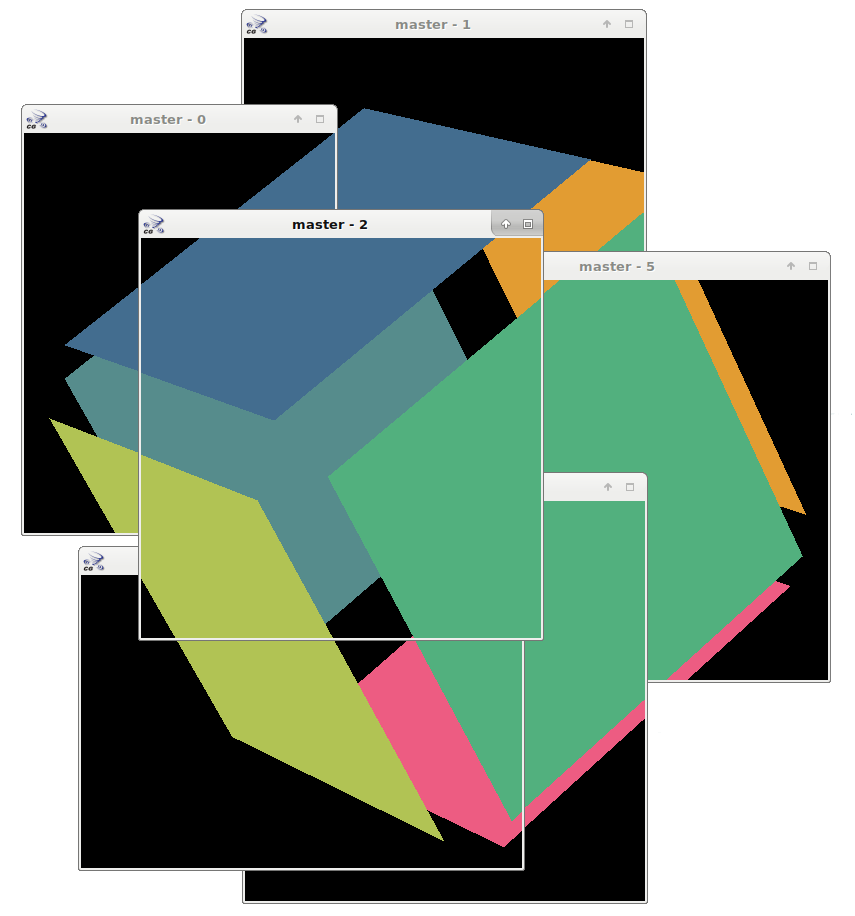
\includegraphics[width=\textwidth]{./fig/minimal-result-0.png}\\
\end{minipage}\hfill
\begin{minipage}{.3\textwidth}
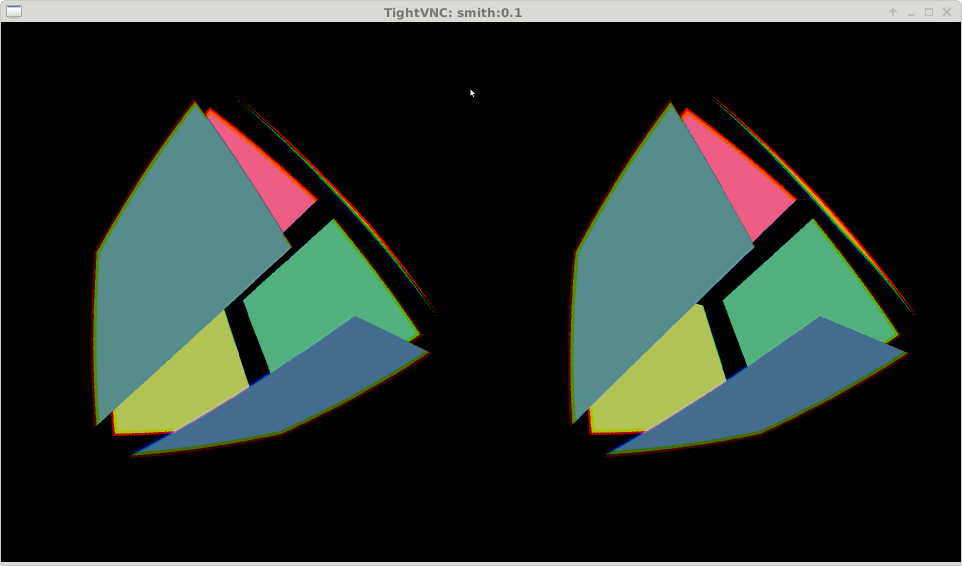
\includegraphics[width=\textwidth]{./fig/minimal-result-1.png}\\
\end{minipage}\hfill
\begin{minipage}{.3\textwidth}
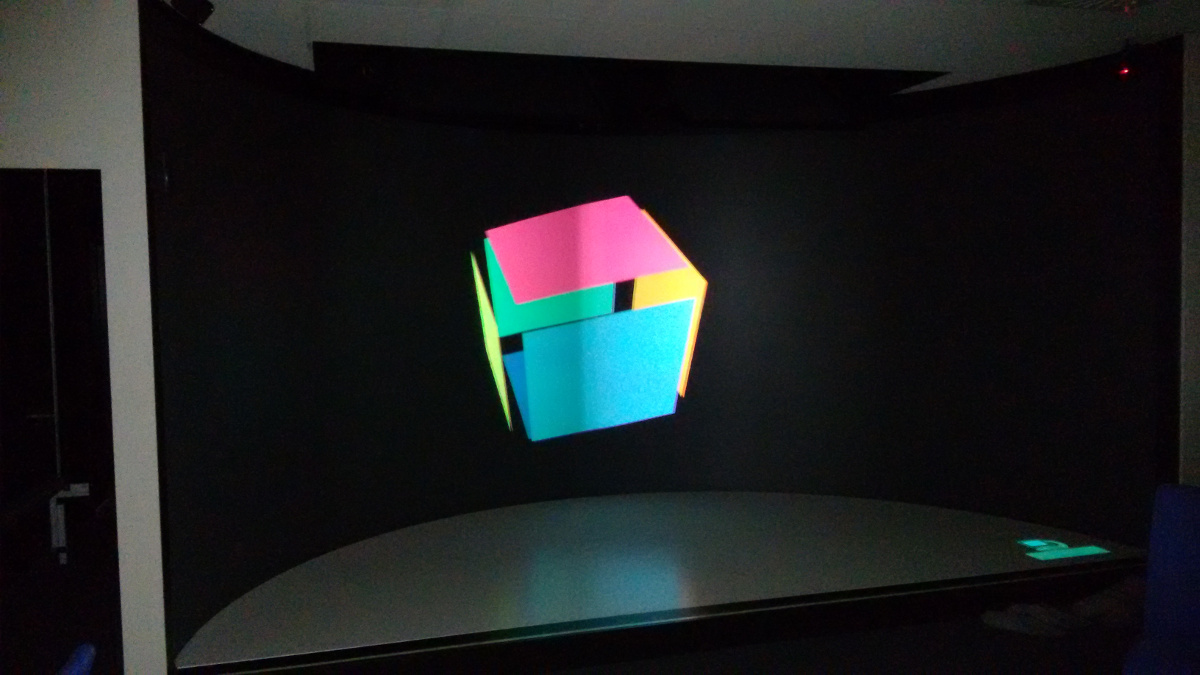
\includegraphics[width=\textwidth]{./fig/minimal-result-2.jpg}\\
\end{minipage}\\
\begin{minipage}{.3\textwidth}
\centerline{Desktop Test}
\end{minipage}\hfill
\begin{minipage}{.3\textwidth}
\centerline{Oculus Rift}
\end{minipage}\hfill
\begin{minipage}{.3\textwidth}
\centerline{VR Lab}
\end{minipage}
\end{frame}

\section{QVR Outlook}

\begin{frame}
\frametitle{\insertsection}
What else is there?
\begin{itemize}
\item Support for VR hardware:
    \begin{itemize}
    \item HTC Vive via OpenVR
    \item Oculus Rift via Oculus SDK
    \item Google Cardboard and Daydream via Google VR NDK
    \item Tracking / interaction devices via VRPN
    \end{itemize}
\item Output plugins for arbitrary postprocessing of views
    \begin{itemize}
    %\item Specified in configuration file; application does not know
    \item Edge blending, warping, color correction for multi-projector setups
    \item Special stereo output modes not covered by QVR
    \end{itemize}
\item Example programs
    \begin{itemize}
    \item \href{https://git.marlam.de/gitweb/?p=qvr.git;a=tree;hb=HEAD;f=qvr-example-opengl-minimal}{qvr-example-opengl-minimal}: rotating cube
    \item \href{https://git.marlam.de/gitweb/?p=qvr.git;a=tree;hb=HEAD;f=qvr-example-opengl}{qvr-example-opengl}: simple demo scene with ground floor
    \item \href{https://git.marlam.de/gitweb/?p=qvr.git;a=tree;hb=HEAD;f=qvr-example-openscenegraph}{qvr-example-openscenegraph}: full-featured \href{http://www.openscenegraph.com/}{OSG} viewer
    \item \href{https://git.marlam.de/gitweb/?p=qvr.git;a=tree;hb=HEAD;f=qvr-example-vtk}{qvr-example-vtk}: \href{http://www.vtk.org/}{VTK} visualization pipeline
    \item \href{https://git.marlam.de/gitweb/?p=qvr.git;a=tree;hb=HEAD;f=qvr-sceneviewer}{qvr-sceneviewer}: viewer for many 3D model and scene files
    \item \href{https://git.marlam.de/gitweb/?p=qvr.git;a=tree;hb=HEAD;f=qvr-videoplayer}{qvr-videoplayer}: a video screen for 2D and 3D videos
    \item \href{https://git.marlam.de/gitweb/?p=qvr.git;a=tree;hb=HEAD;f=qvr-vncviewer}{qvr-vncviewer}: \href{https://en.wikipedia.org/wiki/Virtual_Network_Computing}{VNC} viewer (display remote desktops)
    \end{itemize}
\end{itemize}
\end{frame}

\begin{frame}
\frametitle{\insertsection}
How do I get it?
\begin{itemize}
\item Go to \href{https://marlam.de/qvr}{https://marlam.de/qvr}
\item Download the latest version
\item Unpack
\item Make sure you have Qt
\item Build \emph{and install} \texttt{libqvr} first
\item Build the examples and link against the \emph{installed} \texttt{libqvr}
\end{itemize}
\end{frame}

\end{document}
\bye

\begin{frame}
\frametitle{\insertsection}
Terminology
\begin{itemize}
\item A \emph{node} is a computer in a render cluster network.
\item A \emph{process} is a program instance running on a node.
\item A \emph{GPU} is a graphics processing unit attached to a node.
\item A \emph{display device} is a monitor, projector or similar.
\item A \emph{display} is a logical display device that may combine
    multiple physical display devices.
\item A \emph{display screen} is a display part that corresponds to
    a display device.
\end{itemize}
\end{frame}

